\scanpage{79}
\mspage{78}

Mais ça signifie ni plus ni moins que
\[
\bigcup_{\substack{X\in M\\X\unsure{\parallel|\notin}A}}|X|=P\setminus|A|
\qquad\inserted{\text{i.e. }X\in\operatorname{cosupp}A}
\]
% slanted; the note is enclosed in an oval and linked to the following line.
\margin{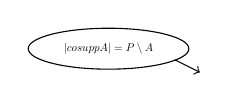
\begin{tikzpicture}[scale=.4,transform shape]
\node at (0,0) {$|\operatorname{cosupp}A|=P\setminus A$};
\draw (0,0) ellipse (2.55 and .65);
\draw[->] (2.1,-.35)--(2.9,-.75);
\end{tikzpicture}}
i.e.\ que l'inclusion $|\unsure{C_M|c_M}(A)|\subset P\setminus|A|$ est une égalité. (En l'occurrence pas seulement pour $A$ $\unsure{\delta|\xi}$ un ensemble support, \unsure{tant} qu'à faire\ldots) Comme $\operatorname{supp}A=\operatorname{cosupp}(\operatorname{cosupp}A)$ on en déduira bien
\[
\begin{aligned}
|\operatorname{supp}A|&=P\setminus(P\setminus|A|)\\
&=A,
\end{aligned}
\]
OK.\ \deleted{$\operatorname{supp}$} Donc

\uline{Lemme 2} Sous les conditions $(\mathrm{iii}_M)$ et $(\mathrm{vi}_M\ \text{a})$, supposons de plus l'hypothèse précédente satisfaite, i.e.
\[
\forall A\subset M,\qquad |\operatorname{cosupp}A|=P\setminus|A|.
\]
Alors pour $\forall A\subset M$, on a
\[
|A|=|\operatorname{supp}A|,
\]
et pour $A,B\subset M$, on a
\diagram{
\begin{tikzcd}[ampersand replacement=\&,column sep=large,row sep=small]
\operatorname{supp}A\subset\operatorname{supp}B
\arrow[r,Leftrightarrow]
\arrow[d,phantom,"{\unsure{\Vert|\Updownarrow}}" description]
\& |A|\subset|B|\\
\bigl(A\subset\operatorname{supp}B
\arrow[d,phantom,"{\Vert}" description]\&\\
\operatorname{cosupp}B\subset\operatorname{cosupp}A\&
\end{tikzcd}
}
\unsure{Cela pour sens|Cela par sens} $\Longleftarrow$ \unsure{connu|comme} dans lemme 1).

L'application (injection, plongement ordonné \inserted{cf Cor. lemme 1})
\[
\Sigma_M\unsure{\mathrel{-}|\longrightarrow}\unsure{\mathcal{P}|\mathscr{P}}(P)
\qquad A\unsure{\mathrel{\vert\!{-}}|\longmapsto}|A|
\]
commute à l'involution $C_M$, $C_P$.
